\documentclass[12pt]{article}
\usepackage[utf8]{inputenc}
\usepackage[cm]{fullpage}
\usepackage{amssymb}
\usepackage{multicol}
\usepackage{graphicx}

\graphicspath{{figs/}}

\newcommand{\exerc}[3]{ \vspace*{25pt} {$\mathbf{#1)}$} #2 \hfill {\it #3} }
\newcommand{\exitem}[2]{ \texttt{\bf #1)} #2 \\ }
\newcommand*\xor{\mathbin{\oplus}}

\renewcommand{\neg}[1]{ 
  \mkern 1.5mu\overline{\mkern-1.5mu#1\mkern-1.5mu}\mkern 1.5mu
}

\newenvironment{exitems}[1]{
\\
\hspace*{30pt}
\begin{minipage}{0.8\textwidth}
\begin{multicols}{#1} 
}{
\end{multicols}
\end{minipage}
}

\newenvironment{exitemss}[1]{
\\
\hspace*{30pt}
\begin{minipage}{0.8\textwidth}
#1
}{
\end{minipage}
}

\begin{document}

\pagenumbering{gobble}

\begin{center}
{\Large \bf Elementos de Lógica Digital - 2015/2}
\end{center}
\vspace{2pt}

{\large \bf 2ª Prova}

{\bf Professor:} Marcos Daniel Baroni

{\bf Data:} 26/11/2015

\vspace{2pt}
{\bf Aluno:} \rule[-2mm]{130mm}{1pt}

\exerc{1}{A partir de três blocos demultiplexadores de 4 canais, projete um
  demultiplexador de 8 canais.}{(2.0 pontos)}
  \begin{center}
    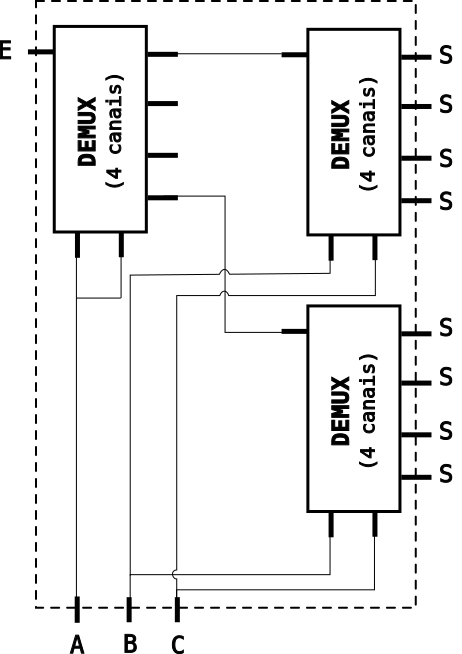
\includegraphics[width=40mm]{demux8}
  \end{center}

\vspace{-14pt}
\exerc{2}{Esquematize o circuito interno de um contador assíncrono que conte de 0 a 9.}{(2.0 pontos)}
\begin{center}
  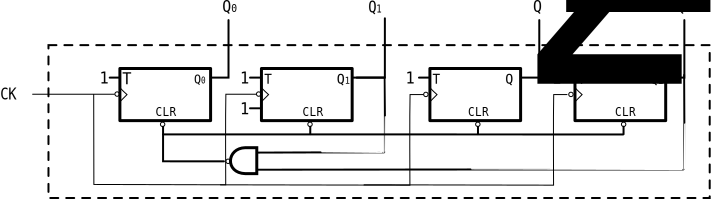
\includegraphics[scale=0.8]{cont3} \\ \vspace{15pt}
\end{center}

%\exerc{3}{Projete um contador síncrono que conte a seguinte sequência:
%$0 \rightarrow 
% 3 \rightarrow
% 4 \rightarrow
% 6 \rightarrow
% 2 \rightarrow
% 5 \rightarrow 0$. Considere que o contador inicia ``zerado''.}{(2.0 pontos)}
\exerc{3}{O contador abaixo realiza a contagem de qual sequência? (considere que
   o contador inicia a contagem ``zerado'')}{(2.0 pontos)}
\begin{center}
  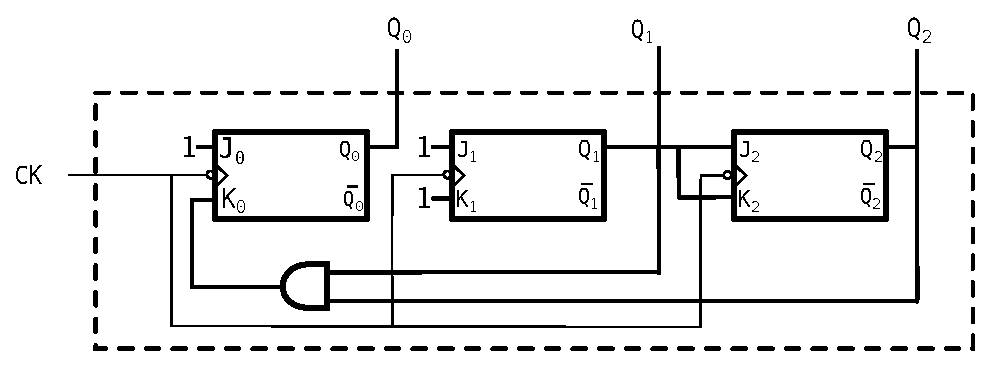
\includegraphics[scale=0.8]{cont2} \\ \vspace{15pt}
\end{center}

\begin{center}
\begin{tabular}{|cccc||cc|cc|cc|}
  \cline{5-10}
  \multicolumn{1}{c}{} & & & & \multicolumn{2}{c|}{$Q_1$} & 1 & 1 & 1 & $Q_1\cdot Q_2$ \\ \hline
  $Q_2$ & $Q_1$ & $Q_0$ & & $J_2$ & $K_2$ & $J_1$ & $K_1$ & $J_0$ & $K_0$ \\ \hline
  0 & 0 & 0 & (0) & 0 & 0 & 1 & 1 & 1 & 0 \\
  0 & 1 & 1 & (3) & 1 & 1 & 1 & 1 & 1 & 0 \\
  1 & 0 & 1 & (5) & 0 & 0 & 1 & 1 & 1 & 0 \\
  1 & 1 & 1 & (7) & 1 & 1 & 1 & 1 & 1 & 1 \\
  0 & 0 & 0 & (0) & 0 & 0 & 1 & 1 & 1 & 0 \\ \hline
\end{tabular}
\\
\vspace{4ex}
$0 \rightarrow 3 \rightarrow 5 \rightarrow 7 \rightarrow 0 $
\end{center}

\vspace{-30pt}
\exerc{4}{Esquematize o circuito interno de uma memória tipo RAM 4x2
  utilizando células básicas de memória.}{(2.0 ponto)}
  \begin{center}
    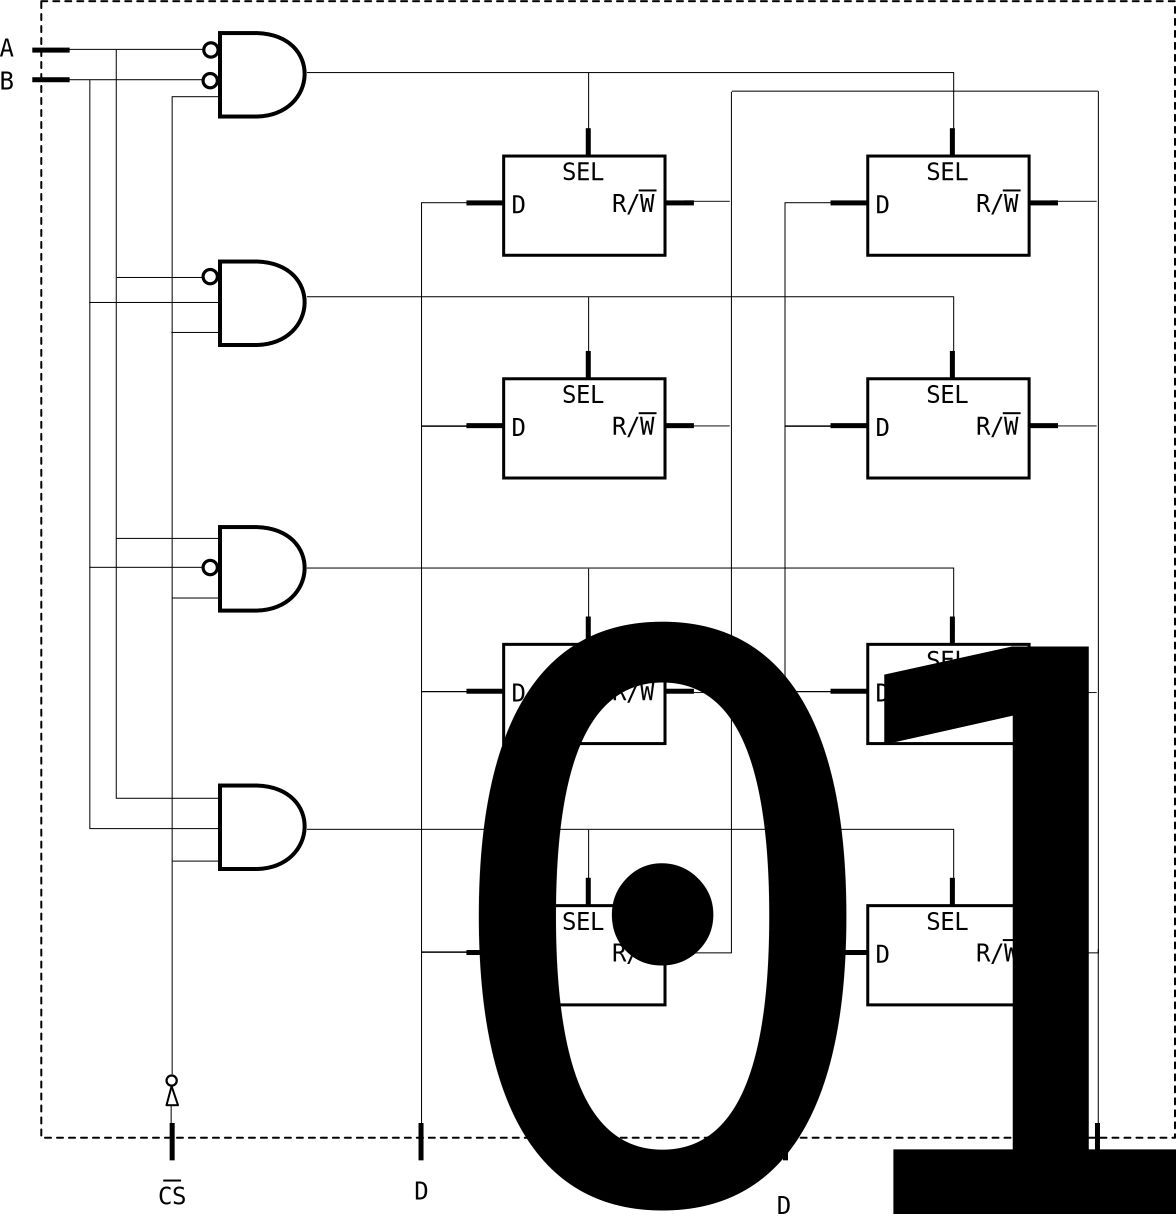
\includegraphics[width=65mm]{mem4x2}
  \end{center}

\vspace{-15pt}
%\exerc{5}{A partir de dois blocos de memória RAM 2x2, realize o projeto
%  de uma memória RAM 2x4.}{(1.0 ponto)}

\exerc{5}{Preencha os atributos de acordo com os modelos de RAM indicados:}{(2.0 pontos)}
\\
\begin{center}
\begin{tabular}{|l|r|r|}
 \cline{2-3}
 \multicolumn{1}{c|}{} & \multicolumn{2}{c|}{\bf RAM} \\ \cline{2-3}
 \multicolumn{1}{c|}{} & {\bf 4M x 4} & {\bf 512 x 8} \\ \hline
 Capacidade total (em bits) & 16M & 4K \\ \hline
 Largura de palavra de dados & 4 & 8 \\ \hline
 Largura da barra de endereços & 22 & 9 \\ \hline
 Palavra de endereço inicial & 00000$_{16}$ & 000$_{16}$ \\ \hline
 Palavra de endereço final & 3FFFF$_{16}$ & 1FF$_{16}$ \\ \hline
\end{tabular}
\end{center}

\end{document}

